%!TEX root = ../dokumentation.tex
\chapter{Grundlagen Laserentferungsmessung}
Um eine Entfernung zu einem Punkt mittels Licht zu bestimmen gibt es verschiedene Möglichkeiten, welche im folgenden Kapitel näher behandelt werden. Ein wichtiger Hinweiß ist zudem, dass im Zusammenhang mit dem Thema \ac{LIDAR} oftmals der Begriff '\acf{ToF}' fällt, dieser beschreibt allerdings nicht immer das direkt damit verbundene Verfahren, sondern allgemein die Entfernungsbestimmung mittels Licht. 
\section{Lichtlaufzeitmessung}
\subsection{Grundprinzip}
Das Grundprinzip der Lichtlaufzeitmessung oder auch \acf{ToF} (Abbildung: \ref{tof}), bezieht sich auf die Zeit, welche ein ausgesandter Lichtimpuls benötigt bis er wieder am Sender eintrifft.\\
\begin{figure}[H]
	\centering
	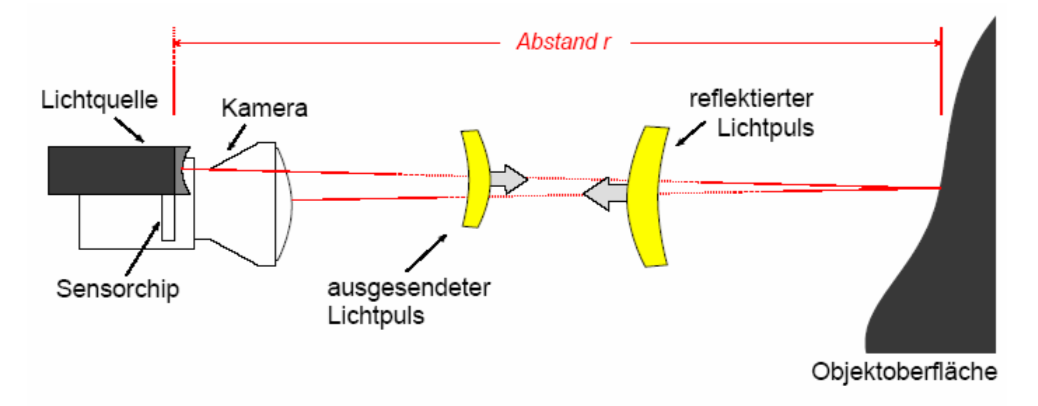
\includegraphics[width=0.75\textwidth]{images/GrundlagenLaserentfernungsmessung/ToF}
	\caption{\ac{ToF} Prinzip \cite{ToF_TUBerlin}}
	\label{tof}
\end{figure}
Dazu wird ein einzelner kurzer Lichtpult von der Lichtquelle ausgesandt, welcher dann von der Oberfläche reflektiert wird und anschließend von einem Sensorchip wieder detektiert werden kann. Über die Zeitdifferenz zwischen aussenden und detektieren des Lichtimpulses und die (halbe) Lichtgeschwindigkeit kann anschließend auf die Entfernung des getroffenen Punktes geschlossen werden. \cite{ToF_ST}
\begin{equation}\formelentry{Berechnung der Entfernung mittels Lichtlaufzeit}\label{lichtlaufzeit}
	r = \frac{t_{diff}}{2} \cdot c
\end{equation} 
\begin{flalign*}
	&r = \text{Abstand zum getroffenen Punkt } \left[m \right]&\\
	&t_{diff} = \text{Zeitdifferenz zwischen aussenden und detektieren des Lichtpulses}\left[s \right]&\\
	&c = \text{Lichtgeschwindigkeit in Luft}\left[\frac{m}{s} \right]&
\end{flalign*}
\subsection{Herausvorderungen}
Bei dieser Technologie entstehen allerdings einige Probleme, auf welche im Folgenden eingegangen wird. Generell sind alle Probleme welche bei \ac{ToF} auftreten miteinander verknüpft, bzw. bedingen sich gegenseitig. \\
Das erste Problem welches Auftritt ist, dass nie das gesamte ausgesandte Licht zur Detektion zur verfügung steht. Durch verschiedene Reflexionsgrade verschiedener Oberflächen und die generelle Streuung des Lichts bei auftreffen auf eine Oberfläche wir immer nur ein geringer Teil direkt zum Sensor zurückgeworfen. Daher sind hoch empfindliche Sensoren nötig um eine zuverlässige Detektion zu ermöglichen.
\ac{SPAD} sind für die Anwendung in einem \ac{ToF} \ac{LIDAR} System sehr gut geeignet, vor allem in einer Anordnung zu einem Array, da eine größere Sensorfläche mit gleichbleibender Genauigkeit realisiert werden kann, und somit eine größere Streuung des reflektierten Lichts abgedeckt werden kann. Allerdings ist das Detektieren des zurückgeworfenen Lichts nicht die einzige Herausforderung welche auftritt, denn mit steigender Distanz nimmt die Dämpfung des Lichtimpulses immer weiter ab. Eine Lösung dafür könnte sein eine Stärkere Lichtquelle zu verwenden, dies birgt allerdings große Sicherheitsrisiken und ist daher nur begrenzt möglich. Eine zweite Lösung ist, die maximale Messentfernung zu limitieren, allerdings birgt dies ein anderes Problem dieses und ein weiteres Problem, welches im Zusammenhang mit der minimalen Messentfernung steht, wird anhand eines Beispiels erläutert.\\
Man nehme an, es existiert ein fiktiver \ac{LIDAR} Sensor mit folgenden Werten:
\begin{itemize}
	\item Minimale Messentfernung $d_{min}=1cm$
	\item Maximale Messentfernung $d_{max}=1000m$
	\item Maximale Messfrequenz $f_{max}=150kHz$ 
\end{itemize}
Formel \ref{lichtlaufzeit} kann umgestellt werden, um die Zeiten zu errechnen, welche das Licht für die minimale und maximale Messentfernung benötigt. 
\begin{equation}\formelentry{Berechnung der minimalen und maximalen Zeit}
	\begin{split}
		t = \frac{r \cdot 2}{c}\\
		t_{min} = \frac{0.01 \cdot 2}{299,79 \cdot 10^6} = 667,13 \cdot 10^{-9}\\
		t_{max} = \frac{1000 \cdot 2}{299,79 \cdot 10^6} = 6,6713 \cdot 10^{-6}\\
	\end{split}
\end{equation} 
\begin{flalign*}
	&r = \text{Abstand zum getroffenen Punkt } \left[m \right]&\\
	&t = \text{Zeitdifferenz zwischen aussenden und detektieren des Lichtpulses}\left[s \right]&\\
	&c = \text{Lichtgeschwindigkeit in Luft}\left[\frac{m}{s} \right]&
\end{flalign*}
Anhand des Beispiels kann man bereits erkennen, dass um die gewünschte minimale Messentfernung zu realisieren eine extrem schnelle Schaltung nötig ist, um das Aussenden und Empfangen innerhalb von $667,13ns$ zu detektieren. Die maximale Messentfernung bringt in diesem Fall ein anderes Problem mit sich, welches noch nicht erwähnt wurde. Zwar ist dies nur ein fiktives Beispiel, allerdings muss das Problem trotzdem betrachtet werden. Der Sensor ist mit einer Maximalen Frequenz von $150kHz \rightarrow 6,6667\mu s$ angegeben, allerdings kann mit dieser Frequenz die maximale Messentfernung nicht erreicht werden, da das Licht länger benötigt. \\
Durch dieses Beispiel wurde veranschaulicht, dass verschiedene Faktoren die Grenzen des Sensors festlegen. Die minimale Messentfernung wird definiert dadurch, wie schnell die Schaltung Aussenden und Empfangen detektieren kann. Die maximale Messentfernung wird von Leistung der Lichtquelle sowie Genauigkeit des Sensors definiert. Die maximale Messfrequenz hängt zusätzlich noch davon ab, wie schnell der Sensor die Daten zur Weiterverarbeitung z.B. an einer \ac{UART} Schnittstelle bereitstellen  kann.

\section{Phasenverschiebung}
Das Phasenverschiebungsverfahren macht sich zu nutzen, dass bei einer ausgesandten Elektromagnetischen Welle die Phase immer größer wird bei steigender Entfernung. Durch Aussenden verschieden Frequentierter Wellen kann dann die Phasenverschiebung der Wellen bestimmt werden und daraus die Entfernung.\\
\todo{Phasenverschiebung}
\section{Triangulation}
\todo{Triangulation}